\chapter{more claws}
\lhead[tempest 2000]{}
\label{sec:more_claws}
\lstset{style=68KStyle}

\begin{figure}[H]
  \centering
    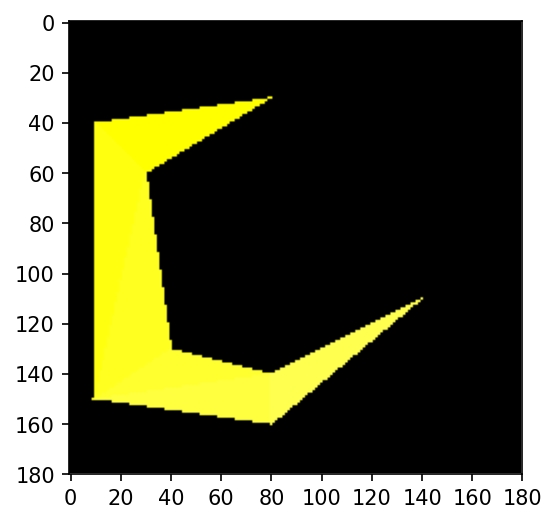
\includegraphics[width=3cm]{build_t2k_claws/final_claw_0_graph.png}
    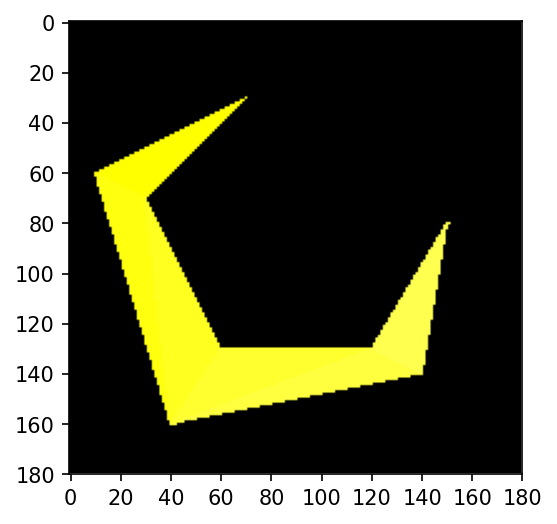
\includegraphics[width=3cm]{build_t2k_claws/final_claw_1_graph.png}
    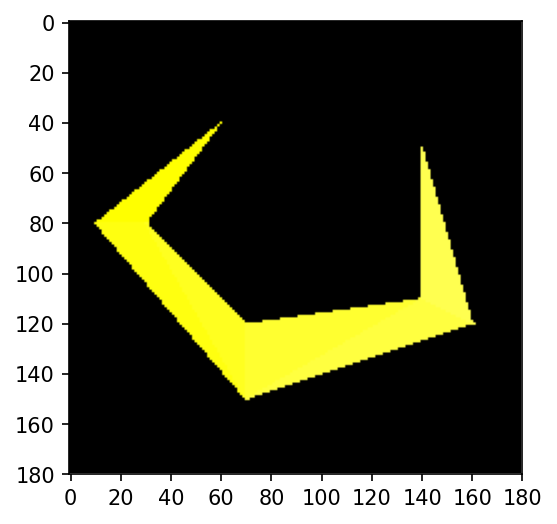
\includegraphics[width=3cm]{build_t2k_claws/final_claw_2_graph.png}
    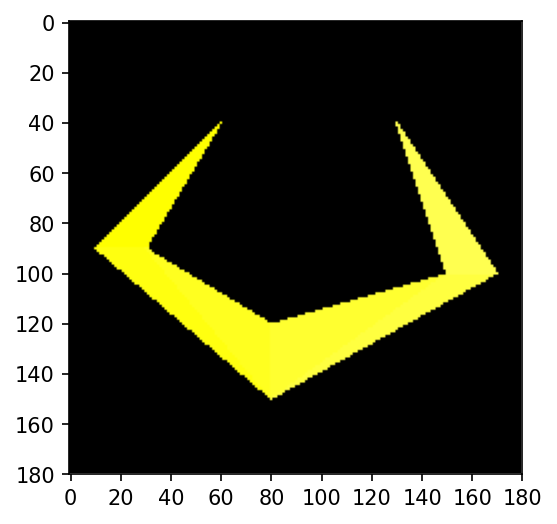
\includegraphics[width=3cm]{build_t2k_claws/final_claw_3_graph.png}
    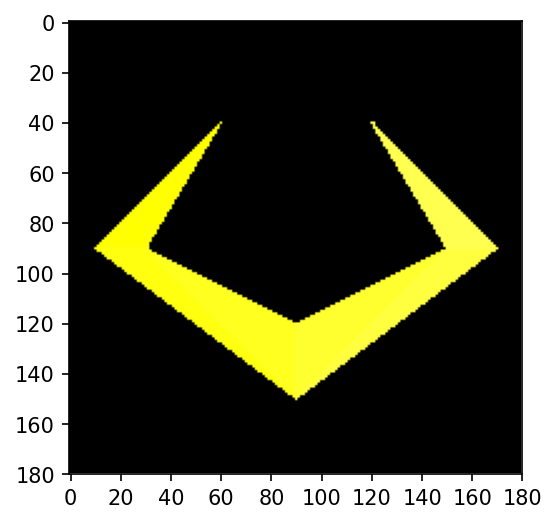
\includegraphics[width=3cm]{build_t2k_claws/final_claw_4_graph.png}
    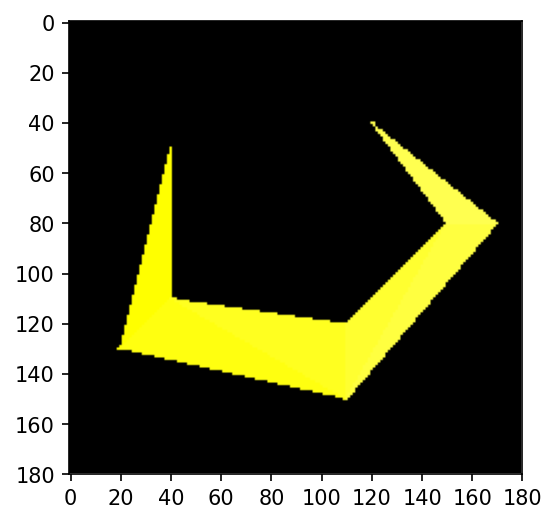
\includegraphics[width=3cm]{build_t2k_claws/final_claw_5_graph.png}
    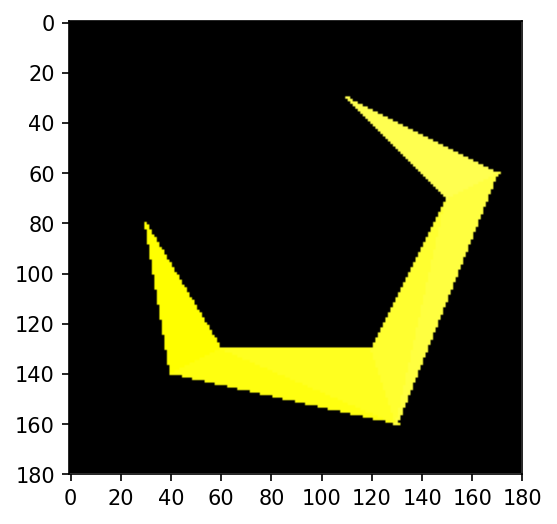
\includegraphics[width=3cm]{build_t2k_claws/final_claw_6_graph.png}
    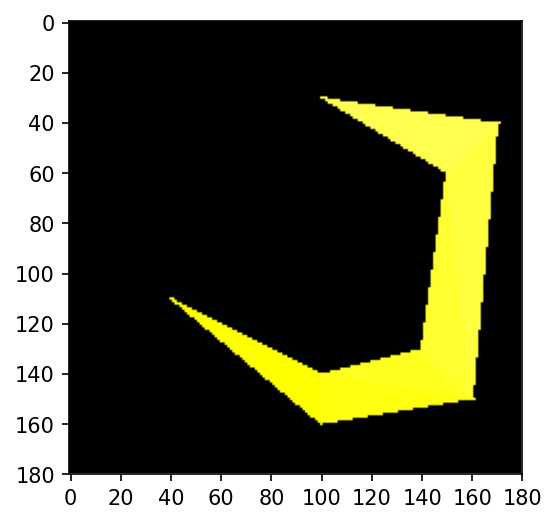
\includegraphics[width=3cm]{build_t2k_claws/final_claw_7_graph.png}
  \caption*{The claws for Tempest 2000.}
\end{figure}

The Tempest 2000 claws are built using the same form of data structure we saw for 
\hyperref[sec:flipper]{\textcolor{blue}{'flippers'.}} So although we don't need to 
rehearse the details in full again here. It is still worth seeing how a claw is built
up from its component polygons.
\clearpage
The data structure for an upright claw in Tempest 2000 mode is as follows:
\begin{lstlisting}
sclaw6:
  dc.l 6              ; 4 faces in this object, a shaded solid Flipper
    
	dc.w $ff            ; Face colour - Yellow.
  dc.w 0,$ff00        ; vertex index, intensity.
  dc.w 1,$ff00        ; vertex index, intensity.
  dc.w 2,$c000        ; vertex index, intensity.
  dc.w 0
    
  dc.w $fe            ; Face colour - Yellow.
  dc.w 1,$ff00        ; vertex index, intensity.
  dc.w 2,$c000        ; vertex index, intensity.
  dc.w 4,$ff00        ; vertex index, intensity.
  dc.w 0
    
  dc.w $fd            ; Face colour - Yellow.
  dc.w 2,$c000        ; vertex index, intensity.
  dc.w 3,$8000        ; vertex index, intensity.
  dc.w 4,$ff00        ; vertex index, intensity.
  dc.w 0
    
	dc.w $fd            ; Face colour - Yellow.
  dc.w 3,$8000        ; vertex index, intensity.
  dc.w 5,$c000        ; vertex index, intensity.
  dc.w 4,$ff00        ; vertex index, intensity.
  dc.w 0
    
  dc.w $fe            ; Face colour - Yellow.
  dc.w 4,$ff00        ; vertex index, intensity.
  dc.w 5,$c000        ; vertex index, intensity.
  dc.w 6,$ff00        ; vertex index, intensity.
  dc.w 0
    
  dc.w $ff            ; Face colour - Yellow.
  dc.w 5,$c000        ; vertex index, intensity.
  dc.w 6,$ff00        ; vertex index, intensity.
  dc.w 7,$ff00        ; vertex index, intensity.
  dc.w 0
    
verts:
	dc.w 3,8            ; Index 0
  dc.w 4,14           ; Index 1
  dc.w 6,13           ; Index 2
  dc.w 12,13          ; Index 3
  dc.w 13,16          ; Index 4
  dc.w 15,7           ; Index 5
  dc.w 17,6           ; Index 6
  dc.w 11,3           ; Index 7
\end{lstlisting}

As before we are constructing our claw with a series of triangles. Each claw
is made up 6 triangles, and for each triangle we specify 3 vertices.

With these, and our specified colour of yellow (\icode{\$ff}), we can make a triangle:

\begin{figure}[H]
  \centering
  \begin{adjustbox}{width=13cm,center}
    \begin{minipage}[c]{0.48\linewidth}
      \begin{figure}[H]
        \centering
        \begin{adjustbox}{width=5.5cm,center}
          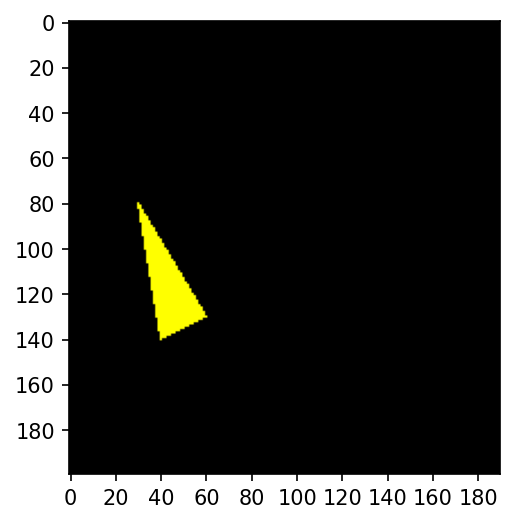
\includegraphics[width=12cm]{src/build_t2k_claws/claw_face_1.png}%
        \end{adjustbox}
      \end{figure}
    \end{minipage}
    \begin{minipage}[c]{0.48\linewidth}
      \begin{lstlisting}[basicstyle=\scriptsize\ttfamily]
dc.w $ff     ; Face colour - Yellow.
dc.w 0,$ff00 ; vertex index, intensity.
dc.w 1,$ff00 ; vertex index, intensity.
dc.w 2,$c000 ; vertex index, intensity.
dc.w 0
      \end{lstlisting}
      \begin{lstlisting}[basicstyle=\scriptsize\ttfamily]
dc.w 3,8    ; Index 0
dc.w 4,14   ; Index 1
dc.w 6,13   ; Index 2
      \end{lstlisting}
      \vspace*{\fill}
    \end{minipage}
  \end{adjustbox}
\end{figure}

\begin{figure}[H]
  \centering
  \begin{adjustbox}{width=13cm,center}
    \begin{minipage}[c]{0.48\linewidth}
      \begin{figure}[H]
        \centering
        \begin{adjustbox}{width=5.5cm,center}
          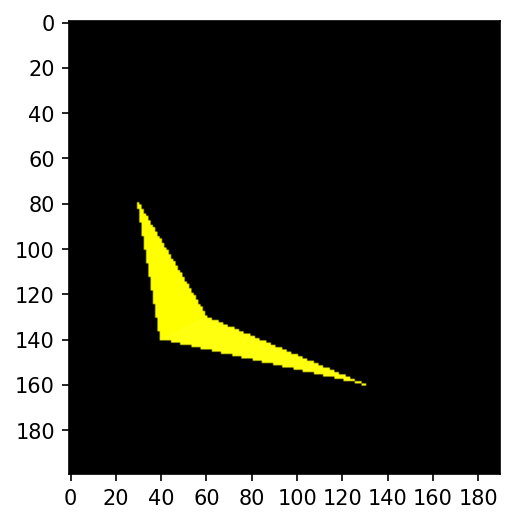
\includegraphics[width=12cm]{src/build_t2k_claws/claw_face_2.png}%
        \end{adjustbox}
      \end{figure}
    \end{minipage}
    \begin{minipage}[c]{0.48\linewidth}
      \begin{lstlisting}[basicstyle=\scriptsize\ttfamily]
dc.w $fe      ; Face colour - Yellow.
dc.w 1,$ff00  ; vertex index, intensity.
dc.w 2,$c000  ; vertex index, intensity.
dc.w 4,$ff00  ; vertex index, intensity.
dc.w 0
      \end{lstlisting}
      \begin{lstlisting}[basicstyle=\scriptsize\ttfamily]
dc.w 4,14   ; Index 1
dc.w 6,13   ; Index 2
dc.w 13,16  ; Index 4
      \end{lstlisting}
      \vspace*{\fill}
    \end{minipage}
  \end{adjustbox}
\end{figure}

\begin{figure}[H]
  \centering
  \begin{adjustbox}{width=13cm,center}
    \begin{minipage}[c]{0.48\linewidth}
      \begin{figure}[H]
        \centering
        \begin{adjustbox}{width=5.5cm,center}
          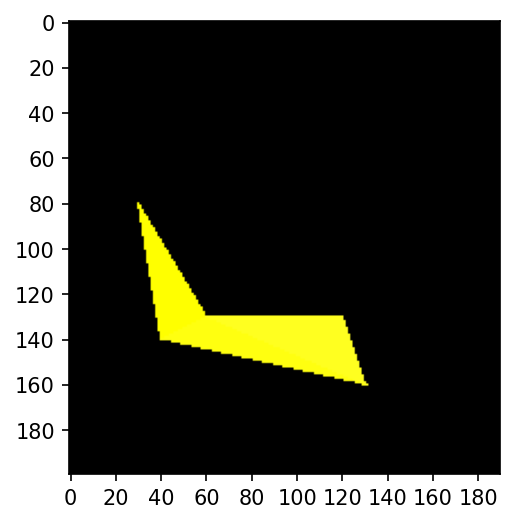
\includegraphics[width=12cm]{src/build_t2k_claws/claw_face_3.png}%
        \end{adjustbox}
      \end{figure}
    \end{minipage}
    \begin{minipage}[c]{0.48\linewidth}
      \begin{lstlisting}[basicstyle=\scriptsize\ttfamily]
dc.w $fd      ; Face colour - Yellow.
dc.w 2,$c000  ; vertex index, intensity.
dc.w 3,$8000  ; vertex index, intensity.
dc.w 4,$ff00  ; vertex index, intensity.
dc.w 0
      \end{lstlisting}
      \begin{lstlisting}[basicstyle=\scriptsize\ttfamily]
dc.w 6,13  ; Index 2
dc.w 12,13 ; Index 3
dc.w 13,16 ; Index 4
      \end{lstlisting}
      \vspace*{\fill}
    \end{minipage}
  \end{adjustbox}
\end{figure}

\begin{figure}[H]
  \centering
  \begin{adjustbox}{width=13cm,center}
    \begin{minipage}[c]{0.48\linewidth}
      \begin{figure}[H]
        \centering
        \begin{adjustbox}{width=5.5cm,center}
          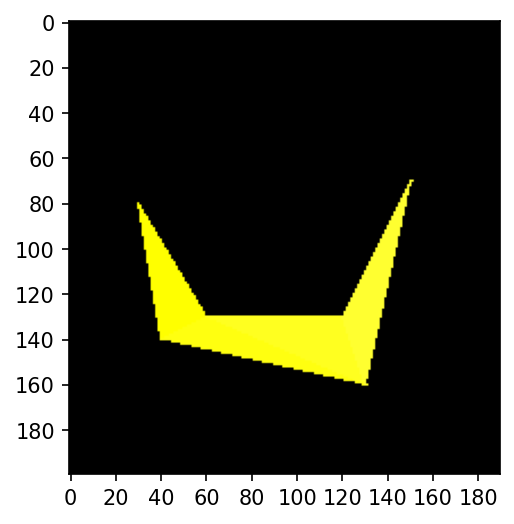
\includegraphics[width=12cm]{src/build_t2k_claws/claw_face_4.png}%
        \end{adjustbox}
      \end{figure}
    \end{minipage}
    \begin{minipage}[c]{0.48\linewidth}
      \begin{lstlisting}[basicstyle=\scriptsize\ttfamily]
dc.w $fd      ; Face colour - Yellow.
dc.w 3,$8000  ; vertex index, intensity.
dc.w 5,$c000  ; vertex index, intensity.
dc.w 4,$ff00  ; vertex index, intensity.
dc.w 0
      \end{lstlisting}
      \begin{lstlisting}[basicstyle=\scriptsize\ttfamily]
dc.w 12,13  ; Index 3
dc.w 15,7   ; Index 5
dc.w 13,16  ; Index 4
      \end{lstlisting}
      \vspace*{\fill}
    \end{minipage}
  \end{adjustbox}
\end{figure}

\begin{figure}[H]
  \centering
  \begin{adjustbox}{width=13cm,center}
    \begin{minipage}[c]{0.48\linewidth}
      \begin{figure}[H]
        \centering
        \begin{adjustbox}{width=5.5cm,center}
          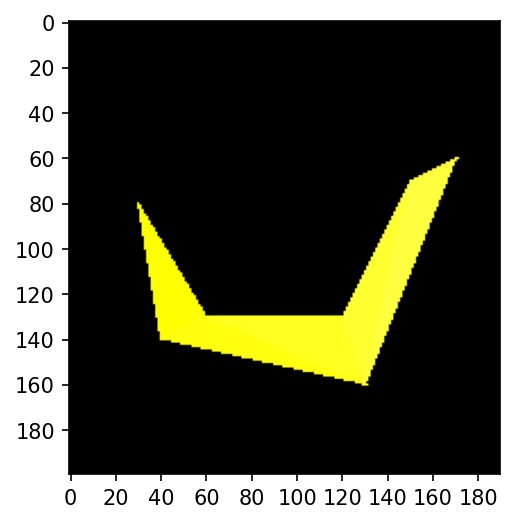
\includegraphics[width=12cm]{src/build_t2k_claws/claw_face_5.png}%
        \end{adjustbox}
      \end{figure}
    \end{minipage}
    \begin{minipage}[c]{0.48\linewidth}
      \begin{lstlisting}[basicstyle=\scriptsize\ttfamily]
dc.w $fe      ; Face colour - Yellow.
dc.w 4,$ff00  ; vertex index, intensity.
dc.w 5,$c000  ; vertex index, intensity.
dc.w 6,$ff00  ; vertex index, intensity.
dc.w 0
      \end{lstlisting}
      \begin{lstlisting}[basicstyle=\scriptsize\ttfamily]
dc.w 13,16 ; Index 4
dc.w 15,7  ; Index 5
dc.w 17,6  ; Index 6
      \end{lstlisting}
      \vspace*{\fill}
    \end{minipage}
  \end{adjustbox}
\end{figure}

\begin{figure}[H]
  \centering
  \begin{adjustbox}{width=13cm,center}
    \begin{minipage}[c]{0.48\linewidth}
      \begin{figure}[H]
        \centering
        \begin{adjustbox}{width=5.5cm,center}
          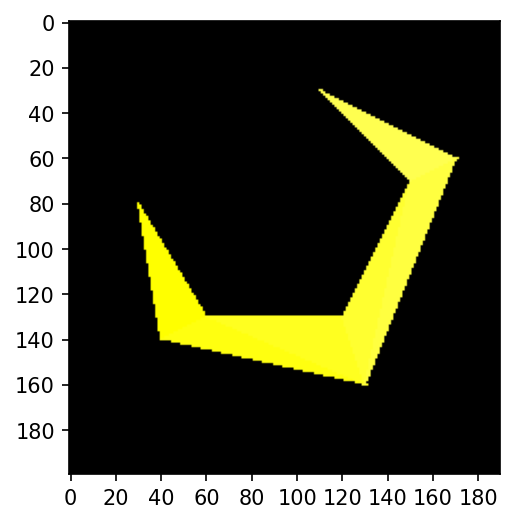
\includegraphics[width=12cm]{src/build_t2k_claws/claw_face_6.png}%
        \end{adjustbox}
      \end{figure}
    \end{minipage}
    \begin{minipage}[c]{0.48\linewidth}
      \begin{lstlisting}[basicstyle=\scriptsize\ttfamily]
dc.w $ff      ; Face colour - Yellow.
dc.w 5,$c000  ; vertex index, intensity.
dc.w 6,$ff00  ; vertex index, intensity.
dc.w 7,$ff00  ; vertex index, intensity.
dc.w 0
      \end{lstlisting}
      \begin{lstlisting}[basicstyle=\scriptsize\ttfamily]
dc.w 15,7 ; Index 5
dc.w 17,6 ; Index 6
dc.w 11,3 ; Index 7
      \end{lstlisting}
      \vspace*{\fill}
    \end{minipage}
  \end{adjustbox}
\end{figure}
